\documentclass[tikz,border=2pt]{standalone}
\usepackage{amsmath,amssymb}
\usepackage{pgfplots}
\pgfplotsset{compat=1.18}

\begin{document}
% Gamma(r, 1) densities for r = 1, 2, 3: the sum of r independent Exp(1) waiting times.
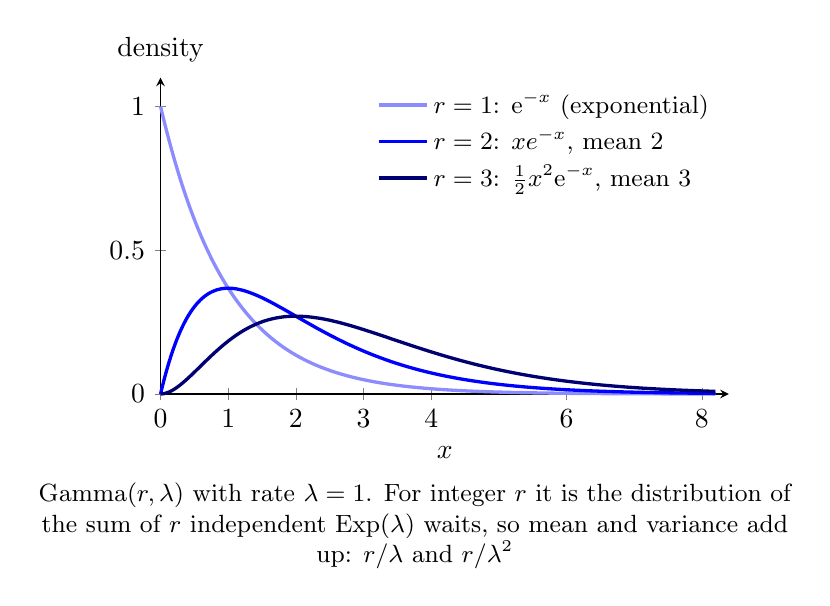
\begin{tikzpicture}
	\begin{axis}[
		axis lines=left, xmin=0, xmax=8.4, ymin=0, ymax=1.1,
		xtick={0,1,2,3,4,6,8}, ytick={0,0.5,1},
		xlabel={$x$}, ylabel={density}, ylabel style={rotate=-90, anchor=south, at={(axis description cs:0,1.02)}},
		samples=140, smooth, width=8.8cm, height=5.6cm, clip=false,
		legend style={draw=none, fill=none, font=\small, at={(0.99,0.99)}, anchor=north east}, legend cell align=left
		]
		\addplot[blue!45, very thick, domain=0:8.2] {exp(-x)};
		\addlegendentry{$r=1$: $\mathrm{e}^{-x}$ (exponential)}
		\addplot[blue, very thick, domain=0:8.2] {x*exp(-x)};
		\addlegendentry{$r=2$: $xe^{-x}$, mean $2$}
		\addplot[blue!45!black, very thick, domain=0:8.2] {x^2*exp(-x)/2};
		\addlegendentry{$r=3$: $\tfrac12x^2\mathrm{e}^{-x}$, mean $3$}
	\end{axis}
	\node[anchor=north, font=\small, align=flush center, text width=9.6cm] at ([yshift=-2pt]current axis.outer south) {$\operatorname{Gamma}(r,\lambda)$ with rate $\lambda=1$. For integer $r$ it is the distribution of the sum of $r$ independent $\operatorname{Exp}(\lambda)$ waits, so mean and variance add up: $r/\lambda$ and $r/\lambda^2$};
\end{tikzpicture}
\end{document}
